\documentclass[11pt]{report}

\parindent 0pt
\parskip 8pt

\usepackage{graphicx}

% reference commands
\newcommand{\fig}[1]{Figure ~\ref{fig:#1}}
\newcommand{\tab}[1]{Figure ~\ref{tab:#1}}

%Gummi|061|=)
\title{Project CS 2012 Course Report\\Uppsala University\\}
\author{Daniele Bacarella\\
Jon Borglund\\
Paolo Boschini\\
Kiril Goguev\\
		Faroogh Hassan\\
		Marcus Ihlar\\
		Alexander Lindholm\\
		Knut Lorenzen\\
		Harold Mart\'{i}nez\\
		Thomas Nordstr\"om\\
		Thiago Costa Porto\\
		Linus Sunde\\
		Kim-Anh Tran
}

\date{}

\begin{document}

\maketitle

\tableofcontents

\chapter{Abstract}
\begin{abstract}
In Information Centric Networking (ICN), content is delivered to users based on
the name of the requested resource without taking into consideration its physical location.
Based on the NetInf protocol, an Android application backed by an Erlang implementation of a
Name Resolution Service was implemented and both products are presented in this report.
By communicating with each other, the systems store, share and retrieve data objects in an ICN fashion.
In situations of network congestion content is difficult or impossible to retrieve.
Using ICN, the system can provide alternate transfer methods to facilitate the delivering of content.
\end{abstract}


\chapter{Introduction}
\chapter{Introduction}

Nowadays the usage of technical devices has become irreplaceable. But with increasing
densification of devices comes network congestion: problems of
browsing the web during a train ride or a concert are apparent. Simply put, the current
location-based networking was not addressed for today's idea of massive content sharing. 
In order to face these problems Information-Centric Networking (ICN) was introduced. For
more information about ICN and all its existing architectures (Data-Oriented Network Architecture (DONA),
Content-Centric Networking (CCN), Publish-Subscribe Internet Routing Paradigm (PSIRP) and Network of Information (NetInf)) 
see \cite{netinf}.
The idea behind ICN is to shift the focus from hosts that serve a content to the actual objects that
are shared. More specifically, these Named Data Objects (NDO) shall no longer be coupled
to a host that is owning the content, but shall ideally be retrievable from \textit{anywhere}.

This report picks a proof-of-concept implementation of the usage of NetInf
(see \sect{netinf}), one out of four concepts that realize ICN. The software was
developed in the context of the 
\textit{Project Computer Science}\footnote{\url{http://www.it.uu.se/edu/course/homepage/projektDV/ht12}},
a course under the supervision of Olle G\"{a}llmo and in cooperation with Ericsson Research \cite{ericsson}
in 2012/2013. The goals set for this project are listed in \sect{goals}. 

The product itself consists of two separate parts developed by two development teams within the same project group. One is an Erlang \cite{erlang} implementation of a Name Resolution Service (NRS) with streaming capabilities.
The other product is a browser application called "Elephant" for Android \cite{android}  phones that takes advantage of NetInf services that
are based on OpenNetInf \cite{opennetinf}, an open source Java implementation of NetInf. 

Both products are described more in detail in \sect{product}. For a thorough understanding
of the implementation and extension of the current state, preliminaries and system architecture decisions are 
described in \sect{preliminaries} and \sect{architecture}. 
The performance of both products are evaluated in \sect{evaluation} and based on the results,
\sect{conclusions} discusses the future work and draws conclusions for the developed products. Finally, the appendix contains installation as well as maintenance instructions.

\chapter{Resources}

\section{Project Group}

\begin{table}
\centering
\begin{tabular}{|l|c|}
\hline
Group member & Nationality \\ \hline\hline
Daniele Bacarella & 
\includegraphics{graphics/it.png} \\
Jon Borglund & 
\includegraphics{graphics/se.png} \\
Paolo Boschini & 
\includegraphics{graphics/it.png} \\
Kiril Goguev & 
\includegraphics{graphics/bg.png} \\
Faroogh Hassan & 
\includegraphics{graphics/pk.png} \\
Marcus Ihlar & 
\includegraphics{graphics/se.png} \\
Alexander Lindholm & 
\includegraphics{graphics/se.png} \\
Knut Lorenzen & 
\includegraphics{graphics/de.png} \\
Harold Mart\'{i}nez & 
\includegraphics{graphics/ve.png} \\
Thomas Nordstr\"om & 
\includegraphics{graphics/se.png} \\
Thiago Costa Porto & 
\includegraphics{graphics/br.png} \\
Linus Sunde & 
\includegraphics{graphics/se.png} \\
Kim-Anh Tran & 
\includegraphics{graphics/de.png} \\
\hline
\end{tabular}
\caption{Each group member's nationality}\label{fig:nationality}
\end{table}

In our project we are 13 students coming from 7 different countries (see \fig{nationality}).
It was a great experience to have team mates from different parts of the globe - not
only working-wise but also food-wise! As our fika rule states, any person who comes later
than 9 o'clock should bring fika for the rest of the group. Thus, we could
try Teque\~{n}os ("cheese sticks") from Venezuela or Tiramisu from Italy.\\

Due the scale of the project, the group decided to divide into two teams. 
The frontend team (LISA), responsible for implementing the client side of the NetInf project and the backend team (ERNI), responsible for implementing the server technology.\\

The groups were divided as follows:

\begin{minipage}[b]{0.32\hsize}\centering
\begin{tabular}{l}
The Frontend team (LISA) \\\hline
Paolo Boschini\\
Harlold Martinez\\
Thiago Costa Porto\\
Linus Sunde\\
Kim-Anh Tran
\end{tabular}
\end{minipage}
\hfill
\begin{minipage}[b]{0.32\hsize}\centering
\begin{tabular}{l}
The Backend team (ERNI) \\\hline
Daniele Bacarella\\
Jon Borglund\\
Kiril Goguev\\
Faroogh Hassan\\
Alexander Lindholm\\
Knut Lorenzen\\
Thomas Nordstr\"om
\end{tabular}
\end{minipage}

Since we had two office rooms, each team could have one of its own.
Nevertheless, we needed to continuously communicate with each other,
since we were working on the same project with the same customer.

\subsection{Seating arrangements}
The seating arrangement of both groups are shown in \fig{frontend_seating} and
\fig {backend_seating}. The main point of the seating within both groups
was to face each other, so that social interaction and communication was facilitated. 

For bigger discussions though, the backend team used the coffee room, whereas the
frontend team had a separate discussion table in the corner of the room. Therefore
other team mates could continue working without being distracted.

\begin{figure}
\centering
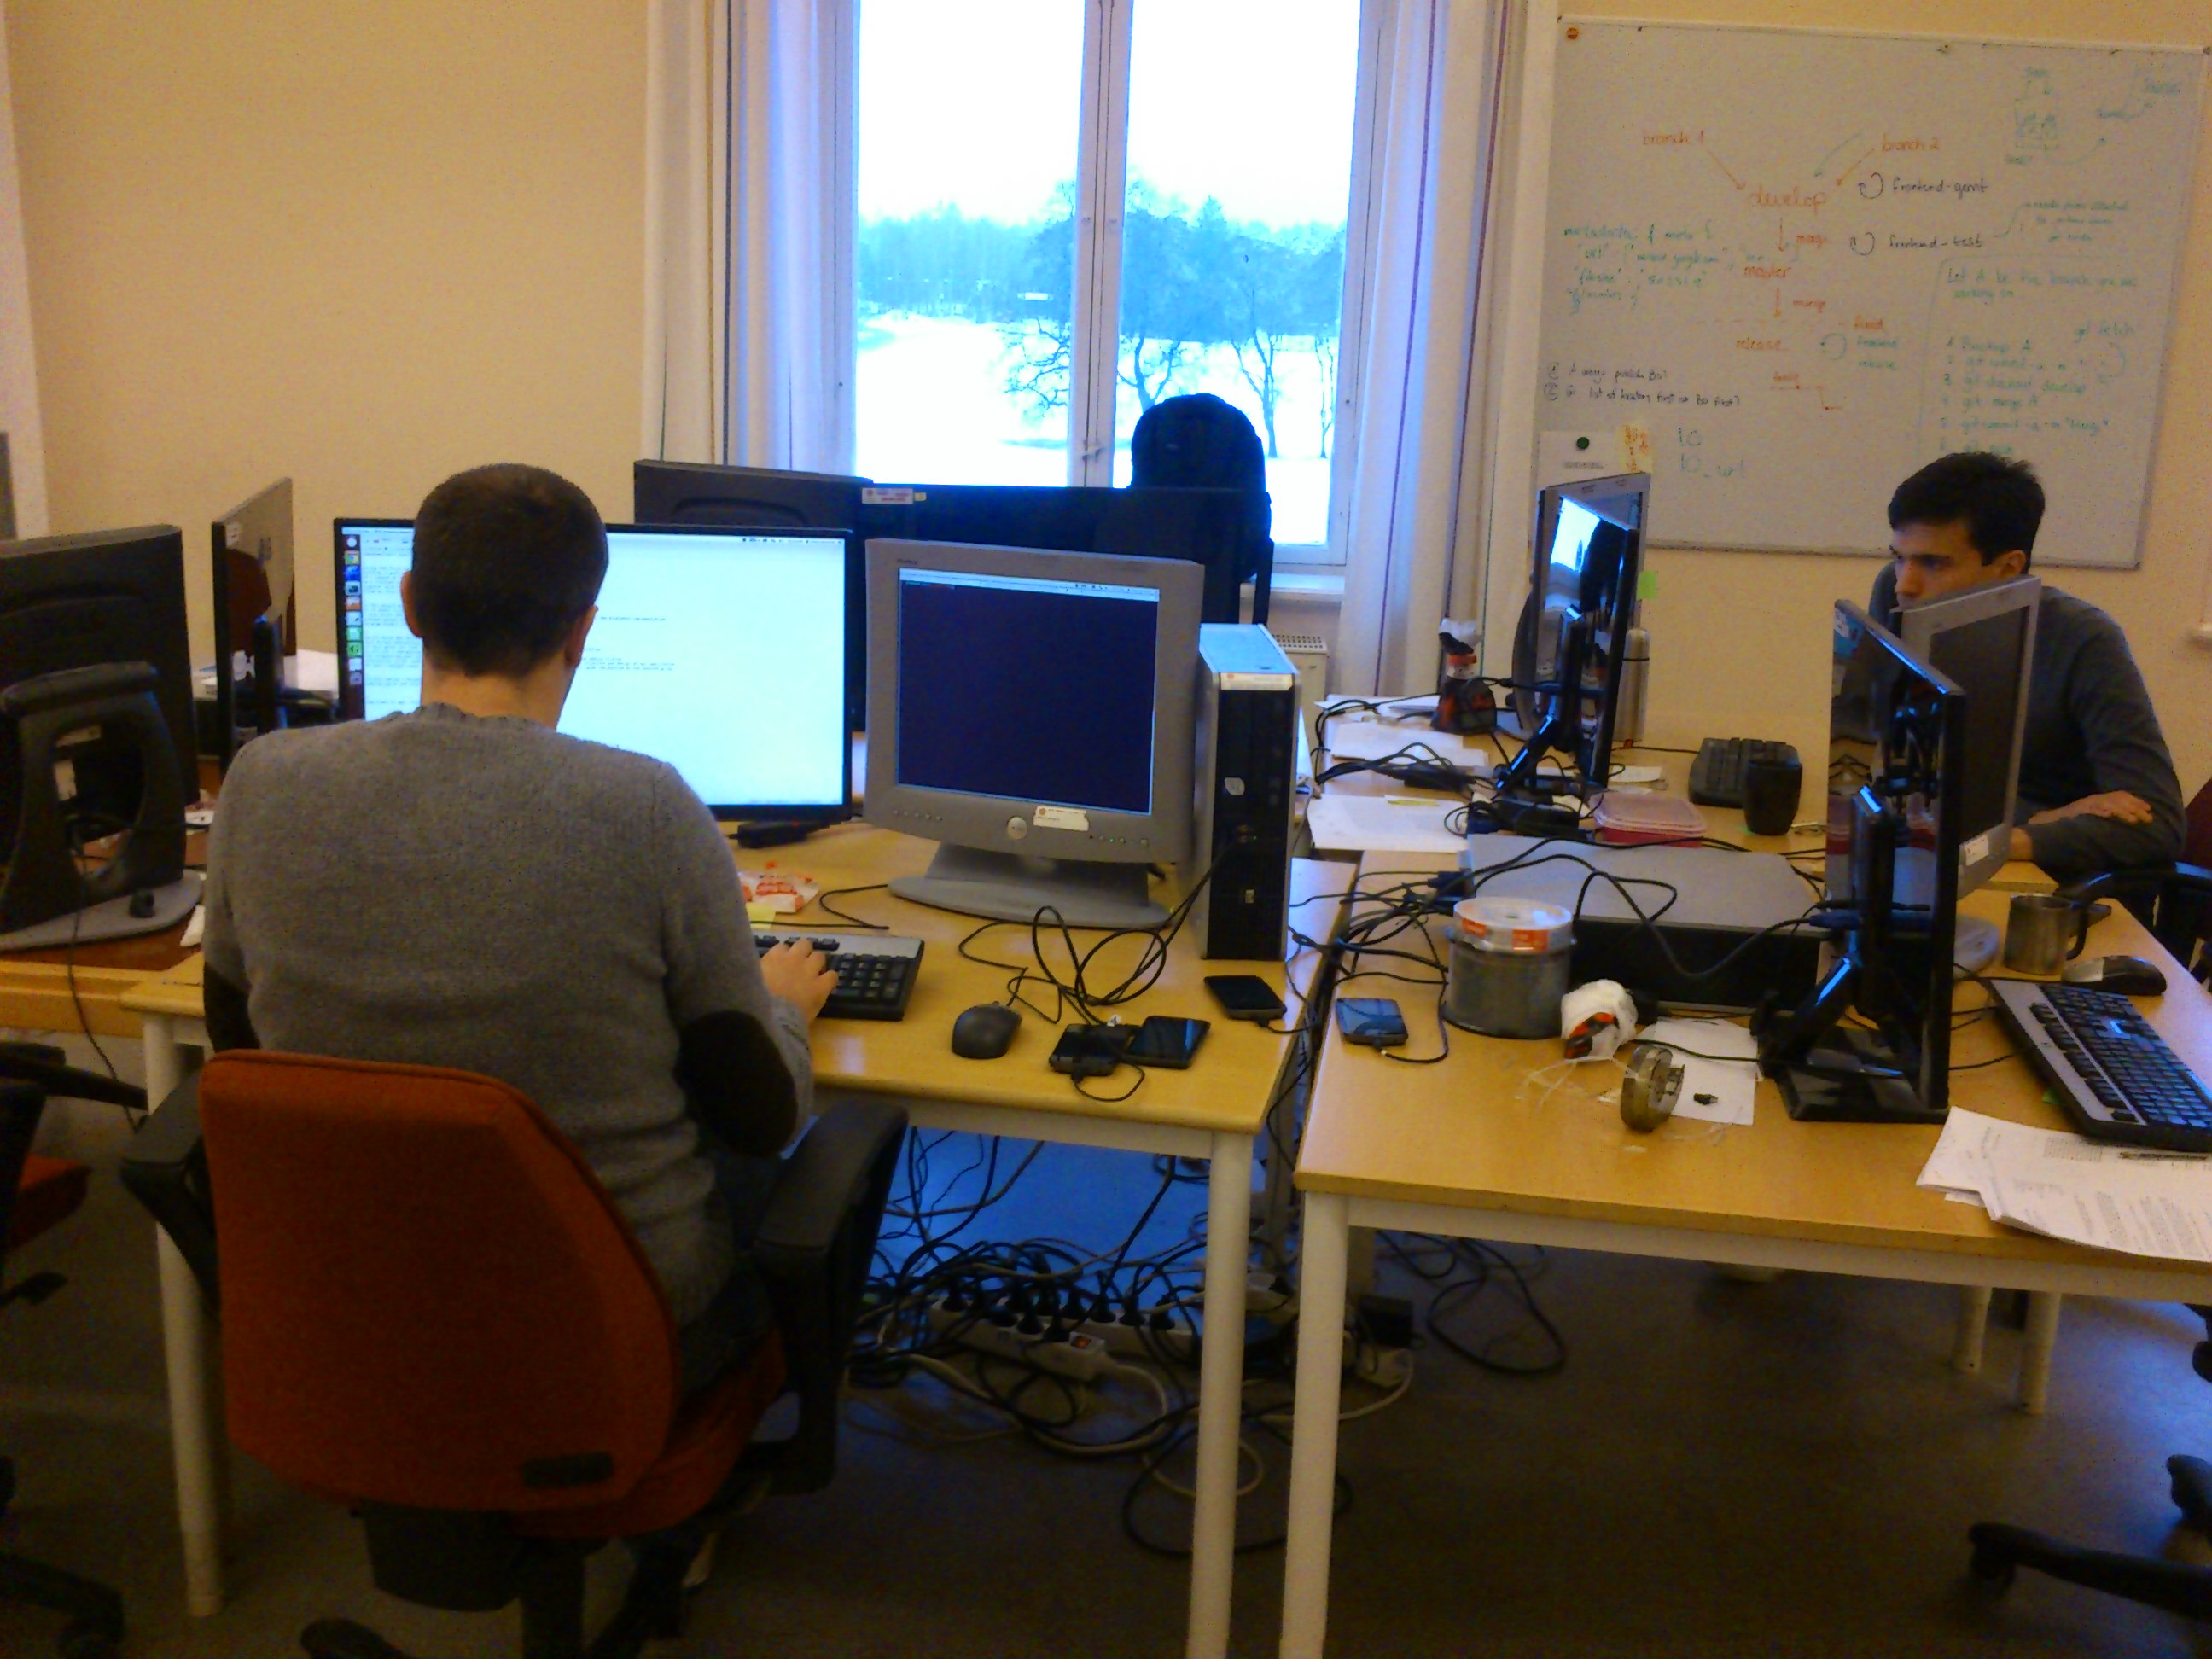
\includegraphics[scale=0.1]{graphics/frontend_seating}
\caption{Frontend seating arrangement}\label{fig:frontend_seating}
\end{figure}


\begin{figure}
\centering
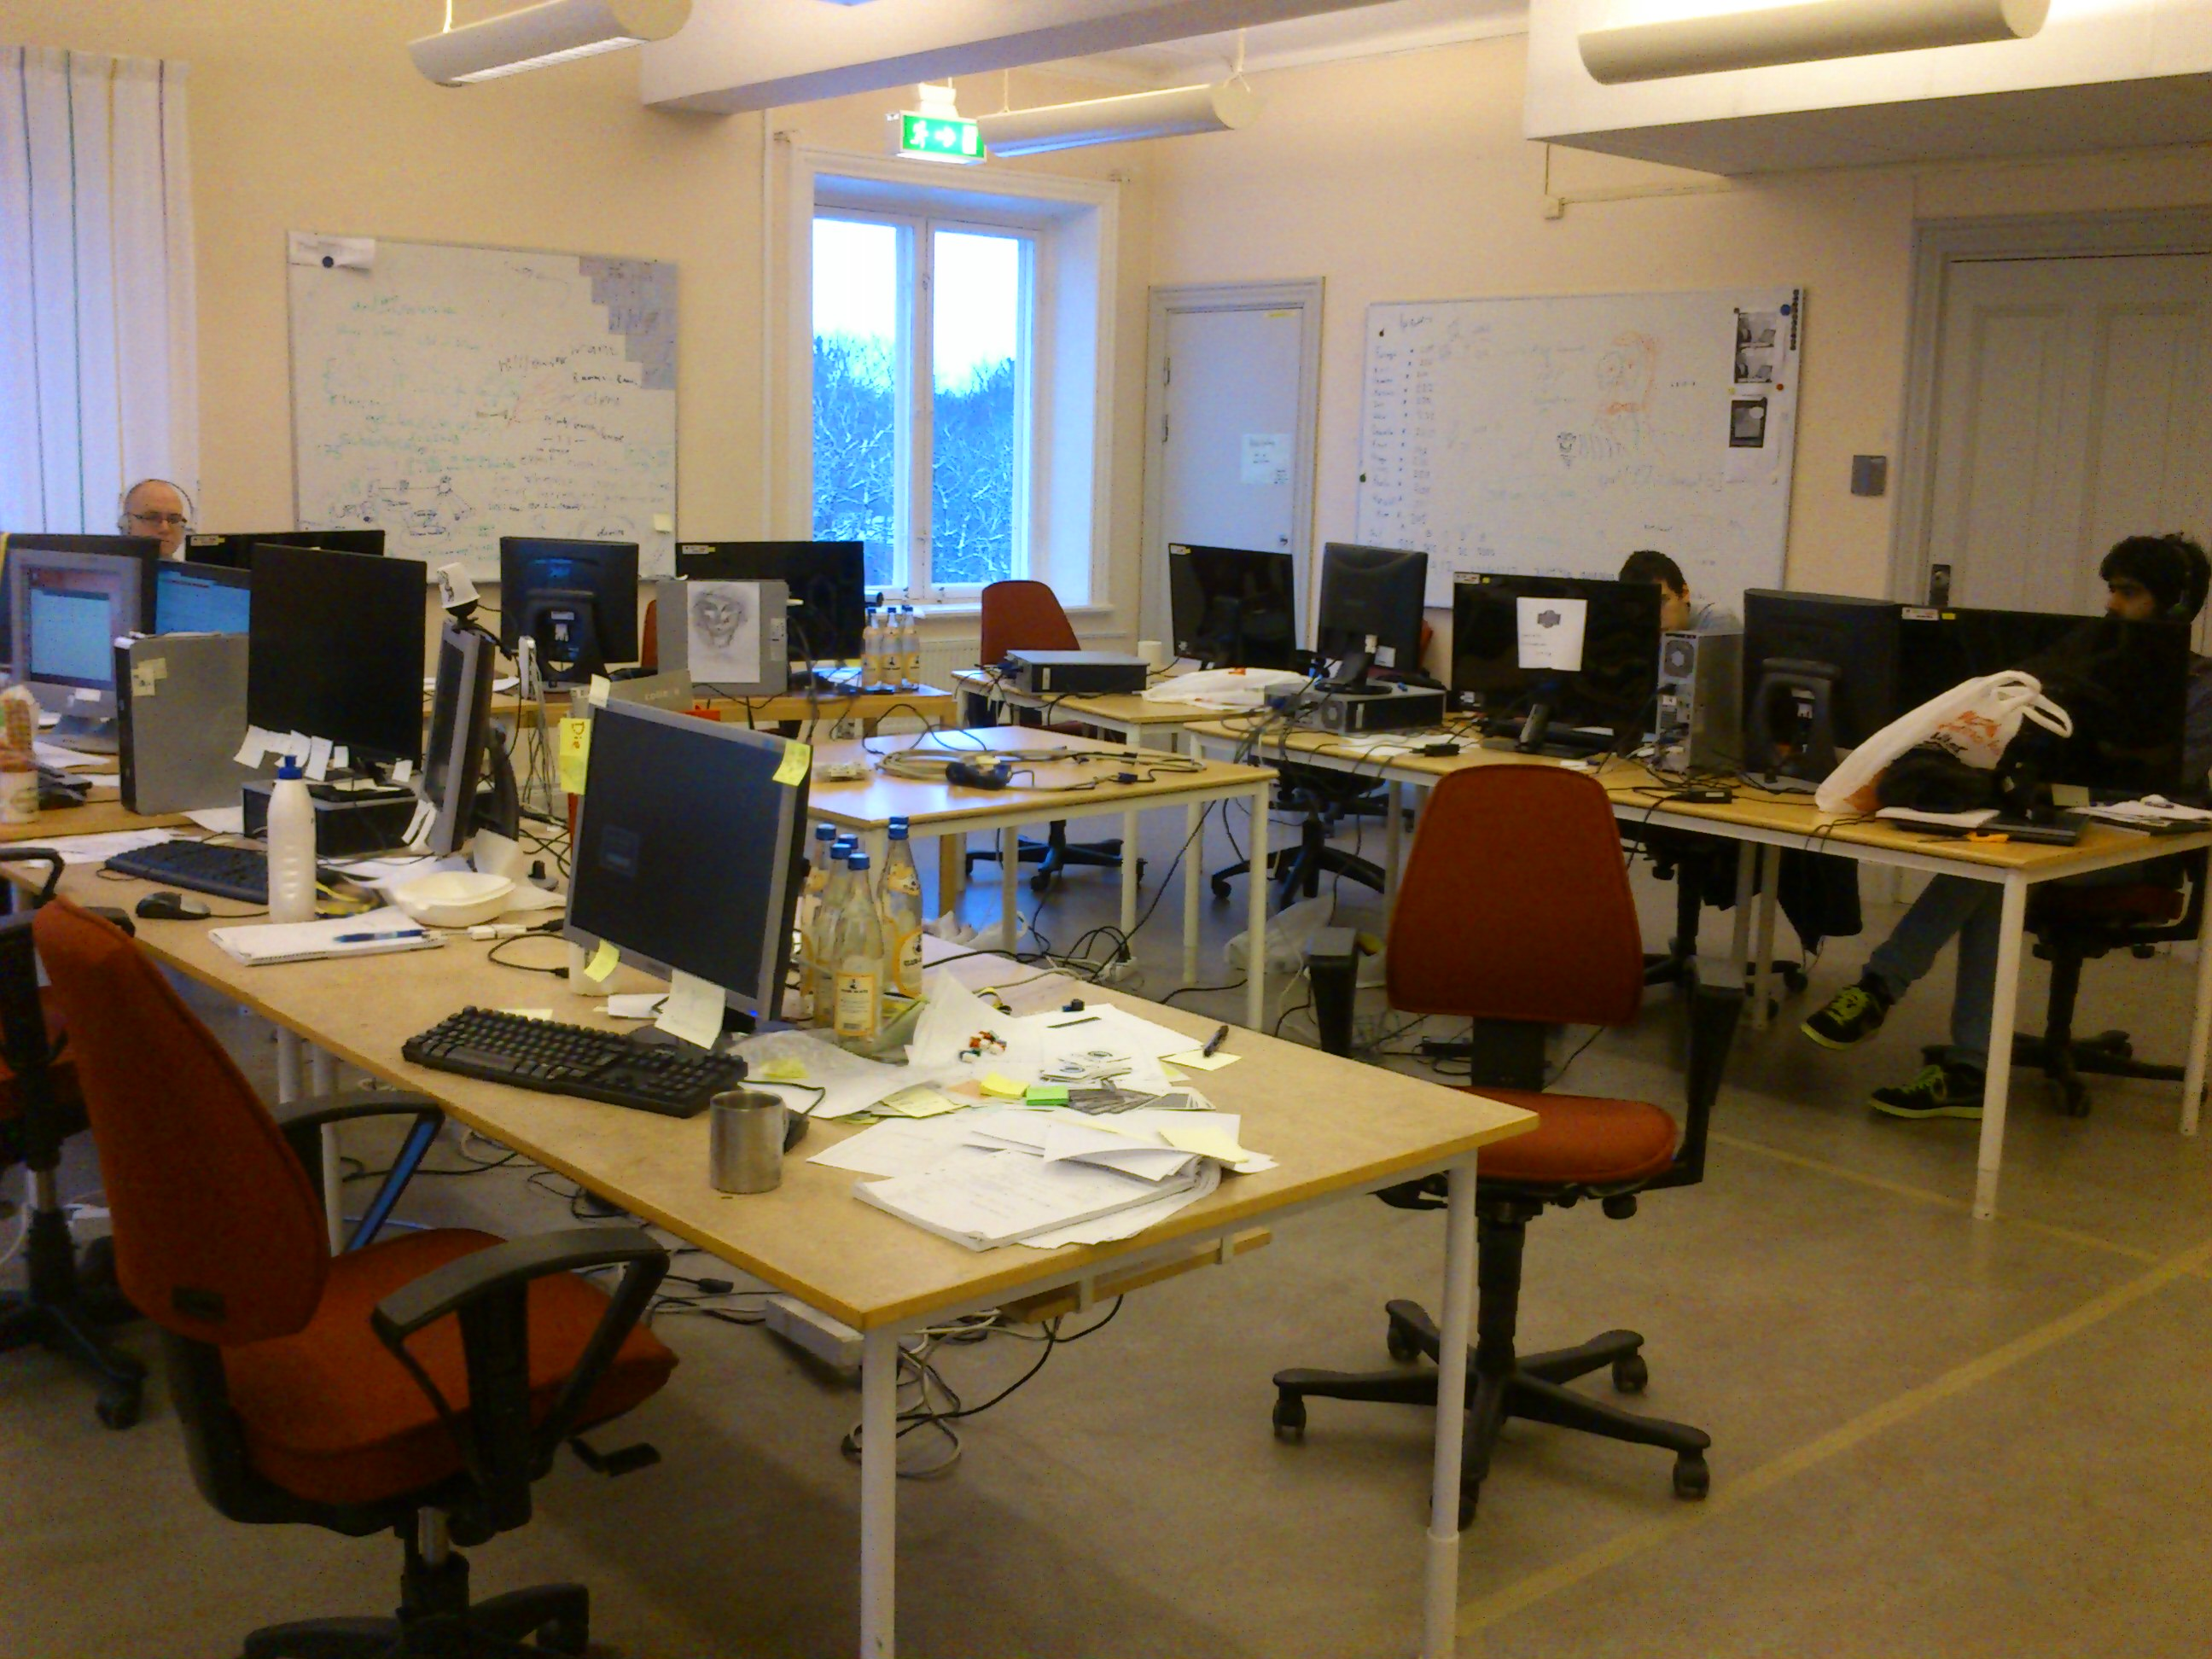
\includegraphics[scale=0.1]{graphics/backend_seating}
\caption{Backend seating arrangement}\label{fig:backend_seating}
\end{figure}



\subsection{Intergroup communication}

\section{Tools}
\subsection{Development Languages}

The LISA team used Android - Java based development language. Their application was targeted at JellyBean Android OS version 1.4.1(Version 16).

The ERNI team used Erlang, Javascript, HTML 5  as their development languages. The main product was coded in Erlang. During the final sprints the client wanted to add video streaming. As a result of this ERNI also created a html client interface to our system using Javascript and HTML 5. 
\subsection{Continuous Integration \& Build Server}

We adopted a continuous integration server which allowed the developers to create special 'jobs' which will control the compilation, error reporting/blaming and source control. Other instances of this project used tools like buildbot but after a long and fruitless effort to make and configure buildbot properly we determined that buildbot was a waste of time and looked into a more powerful/user friendly CI server called JENKINS. 

Jenkins is a CI server with a HTTP interface that allows you setup custom jobs for your project. Things like monitoring a version control system for changes or running command line arguments on the code in your project is easy and user friendly with plenty of tutorials and resources online. We used Jenkins to control both the ERNI and LISA project. 

Jenkins was particularly useful for blaming individuals who 'broke the build'. If Jenkins is configured with the email addresses of all people and a build job fails after someone has updated the source code then, Jenkins will send an email out notifying those who have broken the build and those who are affected(all other collaborators on the current code file which is broken).

We have generated a document which explains how to setup and use Jenkins as we have done in this project. 
\subsection{Version Control}
\label{sec:git}

In order to keep the workflow going at a good pace the teams elected to have version control, which is good practice in all projects. Git was used with a custom workflow shown below. \\

Have a server side repository with 4 initial persistent branches.
\begin{itemize}
\item master
\item staging
\item develop
\item release
\end{itemize}

The following naming convention for temporary branches is adopted: 

\begin{itemize}
\item SprintX.shortStoryName
\end{itemize}

NOTE: The temporary branches will be deleted after each successful merge to the DEVELOP branch.

\subsection {Policies}
\begin{itemize}
\item master\\ \\
The 'master' branch will only contain Demo code. This is the code which contains ONLY the fully tested and integrated stories.  \\\\Tags will be made here under the following convention:\\ \emph{SprintX.shortStoryName} \\\\
This is a Jenkins build tool controlled area - No human user should be operating in this branch. \\Jenkins is responsible for  merging from 'release' to 'master' at the end of a sprint- in order to keep the branches synchronized and provide a fresh clean start for each sprint from working demo code.\\
\item release\\ \\
The 'release' branch will only contain individual stories which are completed and fully unit tested. Here the team can pick and choose which stories to include in a specific demo. This branch is also a Jenkins build tool area. \\Jenkins is responsible for integration testing and merging between 'release' and 'master'
\item develop\\ \\
The 'develop' branch will contain all the code that is able to be compiled on the server and is where the human users will start their personal story branches. Also a Jenkins build tool area, the code here will be considered in a "Story done and compiles but not yet tested" state.\\ Jenkins is responsible for unit testing and merging between 'develop' and 'release'

\item staging \\ \\
The 'staging' branch will contain all the dirty code and is where the human users will push code when finished at the end of the day. Also a Jenkins Build tool area, the code here will be considered as a story is in progress it may be done but it also may not compile. Jenkins will pull all the code from this branch and try to compile it, if it compiles then it will be merged with the 'develop' branch.

\item SprintX.shortStoryName\\ \\
The branch's name will contain the local working code for the specific sprint story followed by a short story name-typically the name written on the post it note for example: Message\_Handler. A merge to the 'develop' branch will mean the story is considered done for the sprint but requires testing by integration tools and Jenkins. This branch will be deleted after the tests are passed and the a successful merge is complete.
\end{itemize}

For instructions on how to utilize this workflow see Appendix B \ref{gitworkflow}.

\chapter{Project methodology and organization}
\section{SCRUM}

The project generally specifies SCRUM project methodology. This is rapidly becoming the standard in companies who develop software and makes sense for students who are about to go into the real world of software development to learn it.

\subsection{Roles}

SCRUM distinguishes between the scrum master, the product owner and the development team.

Scrum master position means an individual who will be responsible for the product in a
particular sprint, as well as liaise between the team and the product owner.
A scrum master is responsible for making sure that the team adhere to the scrum guidelines,
and should never be seen as the boss of the group, but instead as the coach.
She should also make sure that the team is one right track keeping a constant eye at the goal
of the sprint and the definition of 'done' for the different tasks.

Product Owner position means an individual who is considered to be the client in the project.
The person who owns and controls the development of the software with the help of the backlog,
prioritizing features and generally the one who is supposed to give you the direction in sprint planning and demos.

The development team is the set of individuals who are working on the code for the product owner.
The team is responsible for creating increments and releasing a working version of the software
for each sprint.


\subsection{Daily meetings and Sprint planning}

Since we have two teams (ERNI and LISA) we had two distinct sets of meetings and sprints. This meant that we had to bear in mind what the other team was doing since we were supposed to work in sync. One scrum master for each team with constant communication between both teams. 


\subsection{Use of SCRUM in this project}

\subsection{Conflicts}
\chapter{Team Building}
\section{Team Building}

In order to maintain a friendly environment at the work place and to make people
feel comfortable and confident with each other, we arranged a series of activities
which are explained below:

\subsection{Fika}
Fika is a Swedish tradition where people take a break to drink coffee or tea. Every Wednesday one
of each team would bring something to share with the rest of the group. The fika break started at 15.00 
on Wednesdays and it lasted for as long until we could regain our focus on the project. We used this time to get to know each other better and discussed 
everything from politics to weather. Apart from the weekely fika, we sometimes also had the 'late arrival punishment fika',
where anyone who didn't show up on time would arrange an extra fika.

\subsection{Birthdays}
We also used to celebrate birthdays of group members. For this purpose we collected 
money at the start of the project from everyone. This 'birthday fund' was used to buy a cake for the birthday celebration. 
We would then take a break from work to celebrate the birthday of the person and eat the cake with coffee or tea. 

\subsection{Eating out}
Every now and then we used to go to a restaurant or a student nation to eat something for lunch or dinner. Also when the weather 
was nice at the beginning of the project, we arranged an outdoor BBQ which gave the team members the opportunity to spend time with each
other outside of the working environment.
\chapter{Conclusion}
\section{Conclusion}
At the end of this project we can proudly say that this project was a success for us. We achieved almost all the goals that we had set for ourselves at the beginning of the project and during each sprint. Our customer Ericsson Research was also happy with our performance and they offered thesis opportunities to a number of our team members to continue working on the application that we built. 

\begin{itemize}
\item{\textbf{What went well:}}\\
Even though we think that we were not 100 percent efficient with Scrum but it helped us a lot during all stages of this project. The morning Scrum meeting kept everyone updated on the progress of the project. The sprint planning and retrospective meetings gave us the opportunity to participate in meaningful discussions regarding how to build different functionlaties as part of our appliation. We are thankful to the teaching staff for arranging different workhops for us. The Agile, Erlang and Testing workshops by experienced professionals who have been part of the industry for many years were very helpful. 

For those who are going to be working with Erlang in future instances of this course, Erlang OTP in action is a great resource and helped greatly in the beginning of the course. Traditionally the course has a 2 week erlang workshop, we however had 1 week self-study (Erlang OTP in action and the online resource learn you some erlang for great good - http://www.Learnyousomeerlangforgreatgood.com) followed by 2 day Erlang workshop. We believe this was a much better way to handle things since we got to make all the mistakes before and ask valuable questions when the expert came in. 

The weekly fika is also something we would like to recommend the future students to continue. It is a good way to keep a friendly environment in the team and to get to know each other.     

\item{\textbf{What did not went well:}}\\ 
Another thing that we learnt during the course of this project was that not everything is going to be the way we plan it to be. We had problems with estimating the duration of different tasks in almost all the sprints. At times we overestimated the time we assigned for the completion of a particular task and at times we underestiamted it. 

Another problem that we had was to choose the right software tool for a particular purpose. At the beginning of this project we spent too much time on installing and reading about the tools that we never used later because we found a better tool. So it is important to choose the right tool from the beginning to save time and resources. To give an example, we installed Buildbot for continuous integration but found it difficult to learn and manage so we switched to Jenkins instead. So our advice to future students is to spend some time in invstigating what is the best tool that is easy to use and can be learnt quickly.          

\item{\textbf{What can be improved:}}\\
 At times durng this project we built functionalities that we had to scrap later because they were not within the scope of the project. It is important to have a discussion before starting to code anything and have the consensus of the team on everything so that you do not end up building something that would be thrown away later. Communication is very important and team members should not shy away from asking quiestions or demanding clarifications on anything.  
 
The communication with customer is also an important part of any software project and we think that for future instances of this course the customer should be involved more in the project and should provide concrete requirements. In our case even though Ericsson Research was the official customer but at most times we had to act as a customer for ourselves and make decisions that otherwise the real customer has to make. 


\chapter{References}

\appendix
\chapter{Individual input}

\section{Daniele Bacarella}

Sprint 1
I setup my working environment by installing all the software needed to start developing such as the Erlang compiler along with the build tool Rebar and the editor Emacs.
Once the environment was ready I started studying and practicing Erlang while getting familiar with the editor Emacs.

Sprint 2
Kiril and I both worked on the NRS logging and the HTTP handler for the system. Then we researched GIT practices and came up with our own workflow and taught it to the group.
Afterwards I created the inital version of the project Makefile and integrated Rebar into it.

Sprint 3
Jon and I  researched database alternatives to the one already adopted that uses a Erlang internal data structure which is a list of key-value pairs. For obvious reasons it did not represent a valid solution to store data since it did not provide reliability and persistency along with other concurrent features that regular DBMS  provide.
Among the many available options, we chose Riak.
After having set everything up to make it fully working we proceeded writing some tests and the database wrapper for it.
Finally we wrote a install guide on the wiki. 

Sprint 4
The back-end team started working independently from the front-end team on the new NetInf Nrs Streaming feature.
It required us to implement a HTTP client interface to the upcoming NetInf Nrs Streaming.
During this sprint I worked with Alex to create the first prototype of the web interface and the Http client which would communicate with the running NRS to perform the operation requests issued by the user.
We also researched video players suitable for the web page.

Sprint 5
I worked with Alex and Jon fixing bugs and design in the Http client and the web interface.

Sprint 6
I helped Kiril with starting the Product and Course reports as well as finalizing the HTTP client interface with Alex.

Sprint 7
I started writing the Product and Course reports.
\section{Jon Borglund}
During the first sprint I mainly refreshed my functional programming skills and also studied quite a bit of Erlang OTP.
During the first couple of days Faroogh and I compiled some coding standards, and researched Extreme Programming practices which we later presented to the group.

On the second sprint we started the implementation of the NRS. During the first days Alex, Linus and I read and compiled a compact version of the NetInf protocol draft to be sure that both the frontend and the backend would interpret it in the same way. Alex and I also created a curl-script that allowed us to test our NRS according to the draft. 
We then continued to design, implement and test the initial storage module. 
We also started to implement an integration test with Erlang and Eunit.

Sprint 3 Thomas and I fixed some bugs in the message handler and message formatter. Then I joined Daniele to choose and add a persistent database. We first investigated which database alternatives there was. We decided to go with RIAK, hence we proceeded with its installation, configuration and finally testing.

During sprint 4 I was the Scrum master, therefore I spent time on scrum master specific tasks, such as entering stuff into Redmine, updating the whiteboard and burn down chart and also conducted minor conflict mediation. 
Thomas and I defined and implemented interesting state statistics, such as number of active request, number of received request etc. We also went through the NetInf protocol draft again to be sure that we have covered everything in the HTTP convergence layer in our implementation.  Marcus, Knut, Faroogh and I also put down half a day to conduct backlog grooming, to generate new backlog items for the next sprint. 

The team was satisfied with me as scrum master during sprint 4, so during this sprint I was re-elected to fulfil these obligations. 
During sprint 5 I worked mainly with Marcus and the implementation of the streaming. 

I continued to work on the video streaming with Daniele and Alex during sprint 6. After some discussion with Ericsson, we changed some of the streaming, mainly to send the chunks as NetInf messages between the nodes, but without content validation. I also worked some with the HTML5 streaming interface. 
It later turned out that Ericsson also wanted a comparison with the modified chunked data with a pure NetInf streaming solution, I started to implement another HTML5 interface to playback video with pure NetInf while Marcus and Thomas worked on the client backend.

In the beginning of sprint 7 Alex and I finished the HTML5 interface for pure NetInf streaming. Then I conducted an evaluation of the streaming. 
\section{Paolo Boschini}
During the first sprint I was in charge of investigating what mobile phones models
would be a good fit for running the application we would build during the project.
I looked at their specification and chose two models that Ericsson would then provide to us.
As a frontend member I then started working on Bluetooth communication between phones
together with Kim. We managed to get phones sending messages to each other and transfer
files as this was one important feature our application should support.

In the second sprint I studied a previous implementation of NetInf and tried to understand
it in depth to get a valid reference to use during the project. 
I also wrote the code conventions for our workflow. After that I continued working on the Bluetooth implementation
with Kim and implemented programmatic discovering of other devices and the ability to
exchange binary information object (BO) between phones.

In the third sprint I took the role of Scrum Master. I got acquainted with Jira, a digital tool for keeping track of stories and sub-tasks.
To have a more instant overview about the sprint state I also used post-its on the whiteboard in our office making sure to synchronize them with Jira.
I was also responsible for keeping track of the work state of the backend group in order to facilitate the communication between
the two groups. The rest of the time was spent by testing and refactoring. I read up on best practices when following 
test driven methodology in an Android environment and integrated that into our application.
At this point our team felt the need to reorganize and optimize our version control system workflow,
so Kim and I reorganized git branches to simplify our version control workflow.
The refactoring part consisted of adding utility classes, fixing incomplete code comments and adding license
information to our code. I then read up more on Android UI components and refined the UI structure and design of our application.
At last I helped Linus to implement functionalities for fetching and posting data to the NRS cache implemented by the backend group.

In sprint four I helped Kim to separate the main application and the NetInf functionalities into two different projects.
This decoupling was very important since it makes it possible for other developers to develop their own application
and use our existing Netinf Android implementation.
Another important feature was implemented in this iteration, namely the routing of network requests to our Netinf service
when downloading web resources before displaying them into our application. Since each html page contains resources (images, text, videos) we could
save them individually and pass them to our NetInf service as Information Objects (IO).

The last sprint involved minor bug fixes so that our application would support and correctly display a major number of web pages.

\section{Kiril Goguev}

During the first sprint I helped setup the build tool environment(investigating Buildbot with Alex, Faroogh and Jon). Then, I read OTP, attended the Erlang workshop and started to have the grasp of Erlang.\\

In the second sprint, I setup Jenkins with Alex and connected the GIT repositories and created a document on how to set it up from scratch. 
Daniele and I designed and implemented the HTTP Handler and the NRS logging service. Along with creating the GIT practices document and teaching the groups how to use the proper workflow for our project. Finally,
I along with Thomas helped design and implement the foundation of the NetInf protocol( The internal representation of messages in the system).\\


In the third sprint
Faroogh and I migrated all the data and build tools from the old server to a new server(due to errors).
Alex and I fixed merging the meta data in the list database, creating and implementing the plug and play database architecture, abstracting the list database to use the new PNP database architecture and finally the content validation. 
Later, I worked with Marcus to implement content storage and content handler into our system as well as fixing the integration test which was broken when we added all the new modules. 
Finally towards the end of the sprint, Faroogh and I designed and implemented a UDP discovery protocol to be able to find other NRS' on the network.
At the very end of the sprint I started looking into Python SAIL implementation of NetInf but had to abandon it since there was too many problems to fix in order to be able to communicate(this was a problem of the differences in the drafts each implementation followed). 
I Also wrote wiki articles for the plug and play database architecture\\

This is the sprint where I felt that I had a good grasp of Erlang and how to code in the proper OTP way. \\

In sprint 4,
I had a part in designing the very first NetInf video streaming draft along with Faroogh and Knut. 
Later Faroogh and I added truncation to the NRS system and verified that we met all the required components of the netinf protocol draft provided at the beginning of the course by the client. \\

In sprint 5,
I designed a setup/install script.
I also designed and implemented the UDP convergence layer from the draft with Thomas and deprecated the UDP discovery protocol Faroogh and I coded in sprint 3. 
I also took over Faroogh's old task of making the list database persistent. 
Finally, I wrote wiki article on how to use the script and test the UDP convergence layer. \\

In sprint 6,
Alex and I organized the Course and Product Reports into separate files.
Thomas and I made the system configurable using external files( .config files) that can be loaded on the command line at runtime and
I wrote the wiki article for how to write for the reports using the structure we created as well as how to use the configuration files in the system.
Also populated draft sections of the course and product report using all the wiki articles the backend team had written during the course.
Fixed and finalized the setup/install script.\\

Finally in sprint 7,
I reorganized the structure for the reports into folders and showed people how to use the structure.
Wrote parts of the product and course report.\\

\section{Faroogh Hassan}

During the first sprint the whole back-end group concentrated on learning Erlang and Open Telecom Platform (OTP). A two day workshop on Erlang by Henry Nyström of Campanja and another workshop by Gustaf Naeser (Hansoft) on Agile software development were also part of this sprint. I worked with Jon to establish the coding standards which we followed throughout the rest of the project. Me and Jon also investigated if their are any Extreme Programming (XP) practices that we can incorporate in our development methodology and we came up with a set of recommendations. \\

I started the second sprint by taking part in developing the overall design of our application. I also worked with Thomas to write code and some tests for message handler and message parser.\\

Third sprint was the longest sprint of this project (3 weeks) and I got the opportunity to be the Scrum master of the back-end team for this sprint. As a Scrum master my major task was to remove any impediments that may arise during the course of development. I worked with Alex on writing for the search functionality. I also worked with Kiril on the NRS discovery protocol where we used UDP messages for the discovery purpose. Apart from that I also wrote unit tests for the modules where unit tests were missing. \\

In the fourth sprint I was involved in designing the architecture of the streaming video functionality. We wrote a draft specification for this functionality based on the proposed architecture. \\

In the fifth sprint I investigated if our implementation of Netinf protocol is compatible with other implementations. We aborted this task later on customer's request. \\

Sixth sprint was the last sprint before the Christmas break where we made some final adjustments to our application and cleaned up our code. I wrote 'specs' and comments in the modules where they were missing. \\

Seventh sprint was the last sprint of our project and we dedicated the whole sprint to write course and product reports. \\

\section{Marcus Ihlar}
During the first I studied OTP design principles, investigated existing http libraries for Erlang and implemented a simple demo server together with Thomas. We decided to use Cowboy for http handling. The server partially implemented NetInf publish and get functionality.

The second sprint signaled the start of real product development. In the beginning of the sprint I did an overall design of the intended system with Faroogh and Thomas. When actual coding started I wrote a lot of the boilerplate code necessary to setup an OTP application, later I focused on event-handling logic and test code.

In sprint 3 I implemented content storage together with Kiril, after that we focused on getting the integration test working properly. Designed the architecture for forwarding of NetInf messages together with Thomas and Alex. I implemented message id storage (as part of the distribution architecture) together with Thomas and then updated the event handler to handle message forwarding, this led to alot of re-factoring throughout the system, especially to make message passing asynchronous. 

Sprint 4 was short, only one week. I focused on re-factoring and code cleanup, especially in the http message formatting module. We also did some backlog grooming and at the end of the sprint I helped finish the streaming draft.

During the fifth sprint I implemented streaming functionality together with Jon in accordance to the draft written the week before. 

Sprint 6 was my turn to try the role of scrum master. Being scrum master at this point felt very straight forward since we were so far into the project and had a good working environment. I did a lot of bug fixing and work on the integration test. Me and Thomas rewrote some of the streaming code and started implementing pure NetInf streaming. We ended the sprint with a beer and Quake 3 session!

I started sprint 7 by finishing the pure NetInf streaming in order to be able to run evaluation tests. I also worked on presentation, evaluation and reports.
 

 




\section{Alexander Lindholm}
The first few weeks of the project was all about team-building as well as reading up on the subjects ICN and NetInf. The first sprint was mainly about refreshing our functional programing skills as well as setting up all the tools such as git, redmine, jenkins, emacs etc. We also came to certain agreements such as trying to use test-driven-development. 

The second sprint I was involved in the creation of a external protocol draft as well as setting up Jenkins along with Kiril and creating curlscripts for testing of our system along with Jon. Jon and I also created a first naive version of a storage. At the end of sprint two most of us were busy fixing bugs before the presentation at Ericsson in Kista. Here I also spent time on implementing a "beautiful logging system" for the presentation in Kista.

Sprint three started off with the presentation in Kista and it went well. Everyone was pleased with how the presentation went. During the rest of the sprint I mostly worked with Kiril and we were involved in writing a module for validation of hashed content as well as writing code for merging of NDO's in the database aswell as fixing the tests for the storage module. Kiril and I also created the plug-n-play database architecture. Other than that Faroogh and I implemented searching of NDO's within our system.

Sprint four I developed modules for forwarding of messages on the Http convergence layer.
A few days after the sprint had started the backend team started to diverge from the frontend due to several facts;
we were done with the basic NRS functionality in the backend and we were planning on implementing streaming within NetInf, which was something that the frontend didn't have time to do. 
Therefore I mainly worked with Danielle and Jon this sprint and implemented a HTTP-client that would come to be used mainly for streaming, but also worked as a fully functional NetInf-client. 

During sprint five I mainly worked with bug fixing within the system as well as making the HTTP-client more robust and fully functional.

During sprint six we had feature-freezed and my work mainly consisted of fixing bugs as well as refactoring code. A lot of time was spent on fixing a bug that resolved around multipart-Http-data being corrupt after transmission, it turned out that the bug was within Cowboy, the open-source Http-client we used. Kiril and I also created the initial structure for the reports. 

In the beginning of sprint seven I worked with Jon on the implementation of a different version of NetInf-streaming that uses pure NetInf for all transmissions instead of a mix of NetInf-messages along with a content-handler which were used in the previous streaming version. 


\section{Knut Lorenzen}

In the pre-Scrum phase I made two project proposals: One was to integrate NetInf into the Android OS, the other one to start a new NetInf branch in Erlang. As Linux kernel level development was considered tedious the first idea was dropped immediately. The Erlang idea initially received a luke warm response as it did not sound very original compared to other proposals. However our Ericsson contacts mentioned that they would love to see a NetInf implementation in Erlang as it is ``their'' own language, and after a few days more and more group members changed their mind, perhaps because they realised it would be a great opportunity to practise and learn Erlang on a real project.

I became the Scrum master of the backend group for the first two sprints since nobody else volunteered. Having worked as a software developer for a few years after my graduate studies and therefore being more experienced, I felt that I would be more useful in overseeing the development process rather than writing code. During that period I spent my time curating the backlog, reviewing people's tasks, coaching them in working test-driven and setting up and using the development infrastructure. I did not write a single line of code until the third sprint. I also presented the backend group's work during first review at Ericsson after sprint two.

Unfortunately for me (I had really enjoyed being the Scrum master), Olle, the course teacher, requested both teams to appoint new Scrum masters after that, so that others could have the opportunity to practice that role. In the three weeks of sprint 3, my work focussed around creating an integration test. So far, only module tests existed, and the HTTP interface was tested interactively using Curl. I tried hard to convince people to write tests for the (automated) integration test rather than interactive Curl-tests or module tests. I continued to add test cases to the integration test and improve it until the end of the project

In sprint four, I decided to become an additional spokesperson for the backend team. I had the impression that there was a lack of communication between the product owners and us during the previous sprint, i.e. none at all until the demo. This had led to some members implementing features not requested by the product owner. At that point, we had mostly finished implementing the NetInf protocol draft, and the focus of the project changed towards adding streaming functionality. For this, no specification or prior implementation existed. I tried to develop a design draft together with B\"orje, our contact a Ericsson, through email communication. This did not work out very well, and so we decided to come up with our own design and present it at the demo after sprint five.

\section{Harold Martínez}

In the first sprint, I worked defining the code convenctions that we wanted to use. 
We discussed them, refined them and I set up the Eclipse plug-in Chekstyle with the chosen convenctions.
Also, I was selected as spokesperson of the group for the whole project, so I managed the communication 
between the customer and the group.\\

In the following sprint, Kim-Anh, Paolo, Linus and I worked on the first architecture draft. On the other hand,
I worked with Linus on the developed of the earliest version of the Resolution Service that will connect with the 
backend's Name Resolution Service, implementing the get and publish methods.\\

In the third sprint, I prepared together with Knut and Thomas the presentation for Ericsson, I also presented this. 
Then I worked together with Kim-Anh designing the Information Object database that will be used for the 
Local Resolution Service.\\

In the fourth sprint, Linus and I cretaed the settings GUI for the Android application, letting the user to change 
some configurations values. I also set up a GitHub account to share the evolution of our project. In order to improve 
the user experience in the application I separate the Bluetooth discovery process and create a scheduled discovery that 
will be triggered from the moment the application starts and runs every five minutes.\\

In the fifth sprint, I began defining and implementing the Bluetooth Convergence Layer, however, due to time constraints 
and other priorities, this job was not finnished. \\

I was SCRUM Master for the whole group for the last sprint where we wrote these reports. I was also in charge of presenting 
our results at the end of the course.\\
\section{Thiago Costa Porto}
When the project started, I read a few papers about ICN and tried to focus on the issues that we were going to face going forward. We had meetings to decide what our project would be like and I felt I was very active in those days. One thing that helped was my previous experience with Scrum, which lead to greater understanding of it by doing it at the university level, giving you the chance to try things the proper way, so to say. When time came, I chose the frontend team because I thought it would be fun to work on the ``client'', shaping it to the way that we had planned.

I was the Scrum master for the first two sprints. In the first sprint, I set up Jira, our project tracker tool, and did all the things the Scrum master should do. I was very focused on getting Scrum to work, at the same time I coded small features for our client. I focused on the networking side of the client, and spent several hours understanding how Android works and how the code we had at our disposal worked. In the second sprint, I could focus more on developing the application and less on Scrum -- everything was going as it was supposed to go -- and I wrote a few of the classes used on the client's backend. I also provided support for measurements (download/upload) and added early support for metadata during transfers.

On the third and fourth sprints I focused mainly on getting the search functionality to work properly. In the third sprint, I provided a solution that was out of the ``NetInf'' architecture, and I focused on integrating it to NetInf using the Resolution Services on the fourth sprint, together with Linus. Apart from the search, I also refactored some code and helped document our code, helped a little with the design of the database, started user feedback and setting up our revised workflow. In the fourth sprint, I worked a lot with JSON, communication with the NRS and making responses uniform throughout our application, with Linus.

Near Christmas, I defined the Evaluation with the other team members and started working on that. I implemented the logging functionality together with Linus and did some extra refactoring on the side. Close to the finish line, I spent time documenting the code for further usage.

This was a very interesting course because it not only simulates a work environment, but provides a lot of insights on your own behavior and on team management. It is very good working with people from different places and with different backgrounds. I definitely recommend this course.


\section{Linus Sunde}

During the first sprint I attended the Erlang Workshop which was mainly directed towards the backend group. This made it natural for me to work with integration between the groups. Together with Thomas and Marcus I worked on sending NetInf messages using HTTP between our application and their server.

In the second sprint I sat down with Jon and Alex and discussed the protocol draft for the NetInf HTTP convergence layer. This discussion resulted in an initial specification. The frontend group decided to use OpenNetInf in our application. I spent some time incorporating OpenNetInf into our project. After this I worked with Harold to create the Resolution Service which communicates with the backend's NRS. This also involved working together with Thomas and Marcus from the other group to solve integration issues as they popped up. Integration issues kept popping up during all the coming sprints and I spent a huge amount of time working on these, most often together with someone from the other group.

I started sprint three with creating a paper prototype together with Kim and Paolo, in preparation for the first review in Kista. The review went well and I felt the paper prototype really gave us a more concrete feeling of our goal. After the review I looked into speeding up the compile time of our application as it was making testing of small changes slow and painful. I also spent a lot of time refactoring, which in hindsight was time well spent. As for new functionality, I worked together with Paolo creating some setup dialogs and downloading of simple web pages using NetInf, as well as sending and receiving cached files from the backend's NRS. Finally I read up on testing using Android JUnit and created tests for some of my code.

During sprint four I once again spent time refactoring, and once again I feel it was time well spent. I worked with Harold to create a settings menu for our application and to make the program use these settings. I worked with Paolo to create a way for our application to know if files were acquired using the Internet, Bluetooth, the NRS cache, or the database on the phone.

I was Scrum Master during sprint five. I spent some time making sure some backend fixes we needed were implemented by the backend. Other than that I mainly worked on preparing evaluation together with Thiago and Paolo. We implemented logging functionality to be able to gather some statistics for our report.

The last sprint was dedicated to writing the reports.

\section{Kim-Anh Tran}
In the first sprint I read up on JIRA and presented the ways to use
JIRA within our project. Afterwards I mainly worked together with Paolo on establishing
the first Bluetooth communication, so that we could handle file requests from other connected
devices. %%that were answered by file transfers.

During the second sprint Harold, Paolo, Linus and I created the first draft of our architecture using OpenNetInf. Thereafter Paolo and I continued on our previous Bluetooth implementation. We added
the Bluetooth discovery and more importantly the functionality to request and
transfer NetInf NDO between devices.

The third sprint I worked on reconfiguring Jenkins with Git and writing a document on
our git workflow. I added a test project for our code that was run by Jenkins.
Afterwards Harold and I worked together in order to develop a database for storing
NDO and thus a Local Resolution Service.

Sprint four involved separating our current application: one that provides
only the NetInf services and one that contains our application which uses
these services. With help from Paolo I separated the two projects and resolved
all dependencies. Afterwards I joined Paolo in order to finish parsing HTML files
to be properly displayed within our WebView component while using our NetInf services.
%%More specifically, we intercepted the WebView activity in case it attempted to
%%download a resource of a page (such as an image) and instead route the 
%%request to our NetInf services.
During this sprint I was Scrum Master. Amongst other tasks I needed to attend the other group's
stand-up meeting, create the stories and tasks in JIRA and update our Scrum board.
It was a good experience to take the role as a Scrum Master and to organize our Sprint.

Within the last sprint I solved the text encoding problem when displaying 
a number of web pages. I cleaned up our logs so that they were readable and
more useful during debugging. Finally I created a JAR file for
libraries that were used in both applications.


\section{Thomas Nordstr\"om}

Pre-Scrum:
In the first few weeks the entire Project CS team read up on ICN in general and NetInf in particular while trying to decide on what our project would be. We also had team-building exercises.

Sprint 1:
We all set up our working environment and had two workshops, one on Erlang and one on Agile development. I also read up on OTP, did some example programs, helped other team members get a hang of functional programming and worked a little on the simple demo server with Marcus.

Sprint 2:
I worked on the message parsing and handling with Faroogh. I also worked on the first draft of the internal message specification and implementation with Kiril. At the end of the sprint I worked with Linus in the front end to make our systems work with each other.

Sprint 3:
First I did some re-factoring of the code, after that I worked on the search both in the message handling and in the list database. I also worked on the presentation at Ericsson with Knut.

Sprint 4:
This sprint I fixed some minor bugs, added some statistics keeping in the server and worked on the backlog grooming.

Sprint 5:
I started working on UDP convergence layer with Kiril.

Sprint 6:
I started the sprint fixing a lot of minor things and while doing that I found a bug in one of our open source  dependencies and got that fixed.

Sprint 7:
In this sprint the entire group worked on report writing and the final presentation.


\end{document}
